\documentclass[11pt]{article}
\usepackage{enumitem}
\usepackage{amsmath,amsthm,amssymb}
\usepackage{color}
\usepackage{graphicx}
\graphicspath{ {./images/} }

\begin{document}
\date{} 
\title{Lab Report 3\\--\\\large CPE282 Fall 2020}
\author{Brennen Green}
\maketitle

\section*{BCD to Seven Segment Display}
\begin{center}
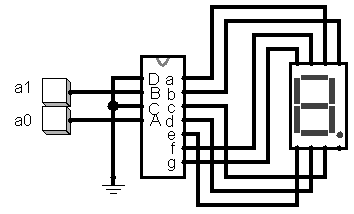
\includegraphics[width=10cm, keepaspectratio]{BCD-7SEG}\newline
\emph{* There should be a 200 $\Omega$  resistor between every pin a-g and the 7-segment display.
I could not find this feature in logisim.}
\end{center}
This design went very smoothly and followed my prelab design spot on. One weird thing that came up
however was that when I plugged in my \emph{first} 7-segment display it worked initially, got very hot,
then started glitching out. I had my lab TA review this and we couldn't find an issue (resistors were being used).
We ended up ditching that original display and hooking up a new one and all of the problems were solved! Other then
that there were no big issues with this design, it made things a lot simpler than desiging a driver by hand. The one
thing to note is that my prelab design did have a slight error in that it did not pins D and C on the BCD. We fixed
this in my final design.
\section*{Black Box Logic}
\begin{center}
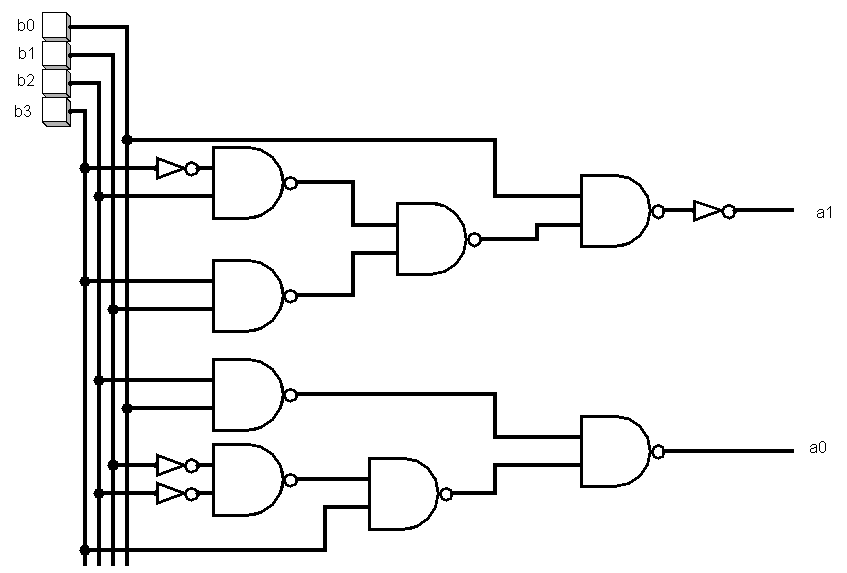
\includegraphics[width=10cm, keepaspectratio]{BlackBox}\newline
\end{center}
Once again this design went really smoothly. After having discovered the amazing use of the 74LS04 inverter chip
last lab wiring these circuit up became a lot easier. I didn't have to deviate from my prelab design what so ever.
However, it was noted that there is a more optimal solution if the goal were to be as optimal as possible.
\newpage
\section*{Final Design}
\begin{center}
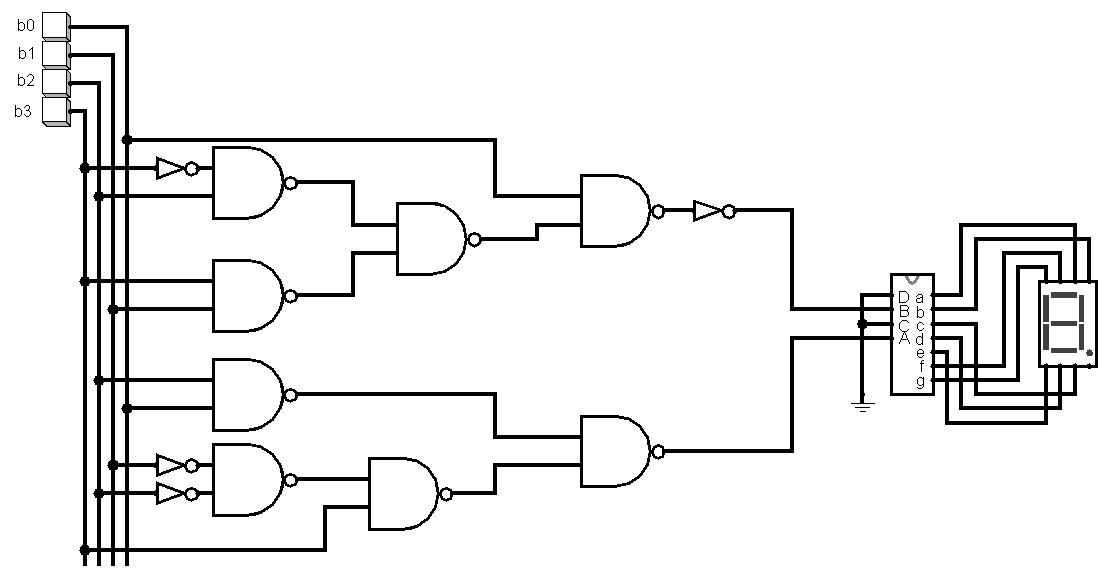
\includegraphics[width=14cm, keepaspectratio]{Final}\newline
\end{center}
In all this lab went really smoothly and I enjoyed it. Despite the weird event that occured with my 7-segment display
burning me originally everything else went according to plan. I've discovered that these integrated circuits such as
the BCD make life a lot easier!
\end{document}

